\section{Data}
\label{sec:data}

\paragraph{Airport observations.}
We use METAR reports for twelve airports from the Iowa Environmental Mesonet archive \citep{iem}:
four in Indonesian Kalimantan (WIOO Pontianak, WAOO Banjarmasin, WALL Balikpapan, WAQQ Tarakan),
five in Malaysian Borneo (WBGG Kuching, WBGS Sibu, WBGR Miri, WBGB Bintulu, WBKK Kota Kinabalu),
and three in Sumatra and the Riau Islands (WIBB Pekanbaru, WIPP Palembang, WIDD Batam)
(Figure~\ref{fig:map}). Palangka Raya, in the most fire-affected province, has no archived METAR
and is absent. We keep reports from 1 January 2015 to 31 December 2025, both routine and special
reports (IEM report types 3 and 4). When an hour has several reports, the last one in that UTC hour
is used, so a correction (COR, \pv{audit.ALL.cor}\% of selected reports) replaces the report it
corrects when both fall in the same hour; \pv{audit.ALL.multi}\% of issue hours had more than one
report. IEM distributes the reports with very little quality control \citep{iem}, and we add only
two rules: visibility is clipped at the 10\,km reporting cap (which removes one erroneous
8000\,km value), and a calm report's direction of 0$^\circ$ is treated as undefined rather than
as a north wind.

\paragraph{Target.}
For each station-hour $t$ with a report, the target at lead time $h\in\{6,24\}$\,h is a
\emph{haze-limited visibility event}: at $t+h$ the reported visibility is below 3\,km, the present
weather contains HZ or FU, and it contains no precipitation or fog code. Hours without a report at
$t+h$ have an unknown target and are dropped, as are reports with visibility below 3\,km whose
present-weather group cannot be parsed. Test labels are never imputed.

The target is an observer-reported marker of haze, not a smoke measurement: HZ is also used for
dust or urban pollution, and reporting practice differs by station and changes over time. The
seasonality points mostly to fire smoke: \pv{audit.ALL.event_jul_nov}\% of event hours fall in
the July--November burning season. Proximity to detections is a weak check here, because almost
every hour has a VIIRS detection within 300\,km in the preceding 72\,h
(\pv{audit.ALL.event_fire300}\% of event hours, \pv{audit.ALL.nonevent_fire300}\% of other hours).
We therefore interpret all results as results about this visibility event, not about smoke
concentration.

\paragraph{Coverage and reporting conventions.}
Report completeness differs sharply between countries (Figure~\ref{fig:coverage}). The Malaysian
stations report almost every hour throughout. The Indonesian stations have long gaps before 2021,
for example 12--15\% of hours at Pontianak in 2016 and 2020. Coding habits also differ: Malaysian
stations use HZ almost exclusively (FU in $<0.1\%$ of reports), while Indonesian stations use FU
more often. Our target accepts either code, and we report results separately by country.

\paragraph{Fire detections.}
We use VIIRS Suomi NPP active-fire detections from the FIRMS yearly country archives for Indonesia
and Malaysia \citep{firms}, restricted to 93--122$^\circ$E, 9$^\circ$S--9$^\circ$N. A single
sensor keeps the detection frequency consistent over the period; mixing in NOAA-20 (from 2018) and
NOAA-21 (from 2023) would change the constellation over time. Every record carries the archive's
\texttt{type} attribute, which the near-real-time feed lacks, so these are processed archive
detections. Their locations and counts can differ from what was available in real time; the
latency analysis below shifts detection times but cannot reproduce that difference. Detections
are thermal anomalies, not confirmed fires, and their absence does not imply the absence of fire
under cloud or thick smoke.

The main analysis uses all detection types, as the deployed model does. Non-vegetation sources
(FIRMS types 1--3: volcanoes, static industrial sources such as gas flares, and offshore
platforms) are a small share of the distance-weighted exposure at most airports but not at all:
\pv{audit.veg.WBGB}\% at Bintulu, next to a liquefied-natural-gas plant, and
\pv{audit.veg.WIDD}\% at Batam and \pv{audit.veg.WBGR}\% at Miri. A sensitivity analysis repeats
the key comparisons with vegetation fires (type 0) only.

\paragraph{Haze seasons.}
Events are highly concentrated in time. Three seasons, 2015, 2019 and 2023, contain most event
hours, with 2015 dominant at almost every station (Figure~\ref{fig:coverage}). Any single temporal
split therefore scores very few independent episodes, which motivates our leave-one-year-out
design (Section~\ref{sec:methods}).

\begin{figure}[t]
  \centering
  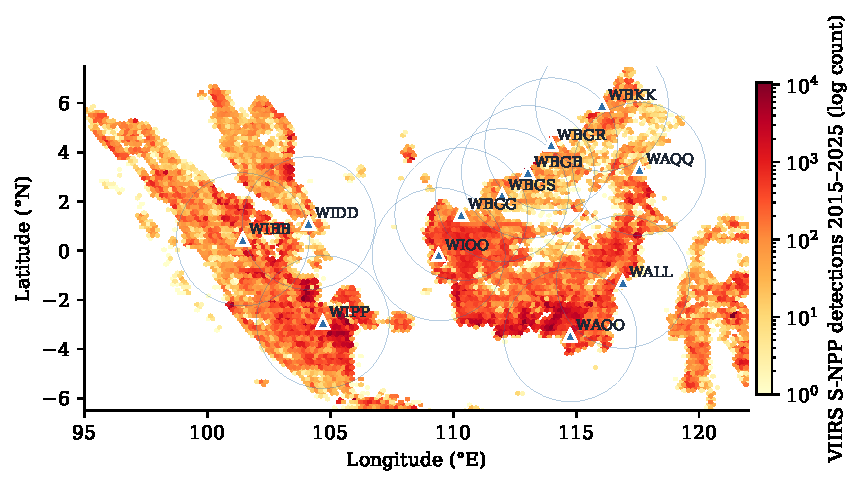
\includegraphics[width=\linewidth]{figures/fig1_map}
  \caption{The twelve airports (triangles) with their 300\,km fire-search radius, over the density
  of VIIRS S-NPP detections 2015--2025.}
  \label{fig:map}
\end{figure}

\begin{figure}[t]
  \centering
  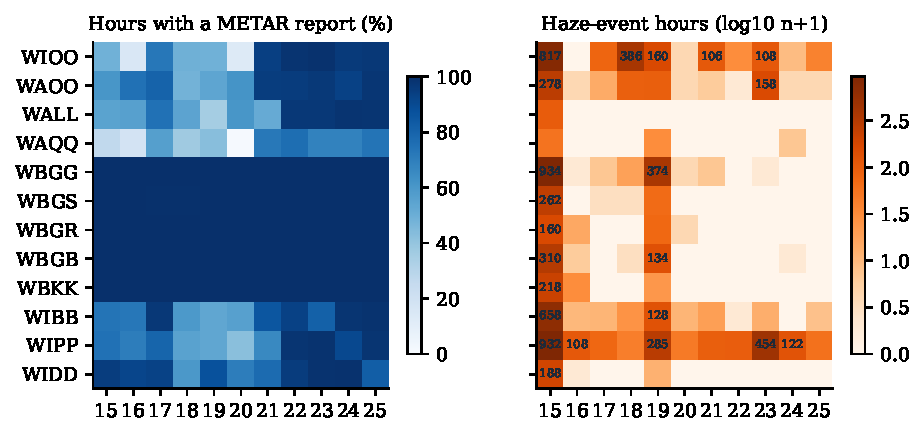
\includegraphics[width=\linewidth]{figures/fig2_coverage}
  \caption{Left: share of hours with a METAR report per station and year. Right: haze-event hours
  per station and year (numbers shown where $\geq 100$).}
  \label{fig:coverage}
\end{figure}
